\documentclass[a4paper, titlepage]{jsarticle}

\date{\today}
\usepackage[dvipdfmx]{graphicx}
\usepackage{url}
% \usepackage[T1]{fontenc}
\usepackage{float}
\usepackage{ascmac}
\usepackage{pdfpages}
\usepackage{enumitem}
\usepackage{otf}

\newcommand{\system}{\textsl{Aero Net}}

\begin{document}
\begin{titlepage}
  \centering
  \vspace*{150truept}
  {\Large 外部設計書}\\
  \vspace*{50truept}
  {\Huge ドローン宅配事業者支援システム} \\
  \vspace{15truept}
  {\Huge \system} \\
  \vspace{50truept}
  {\LARGE 土佐山田IT株式会社}\\
  \vspace{20truept}
  {\large{\tabcolsep = 1cm
      \begin{tabular}{ccc}
        久保田 天治 & 塩澤 康志 & 蝉 祐介  \\
        寺内 俊輔  & 林 晃太郎 & 松本 吏司
      \end{tabular}
    }}
\end{titlepage}

\tableofcontents

\clearpage

\section{機能の概要}

\section{業務フロー図}

\section{機能設計}

\section{ユーザインタフェース設計}

\section{非機能要件 設計}

\section{データ設計}

\section{ネットワーク設計}
図\ref{fig:network}は,本システムのネットワーク構成を示したものである.
本システムは,Amazon Web Services(AWS) の Amazon Cloud Front を用いて作成する.
Amazon Virtual Private Cloud(Amazon VPC) を用い,2つのアベイラビリティゾーン間でのトラフィックの共有を行う.

インターネットゲートウェイにより,各アベイラビリティゾーンへと通信を分散させ,サーバと管理者・事業者・利用者がそれぞれ通信を行う.
各アベイラビリティゾーン内では,Amazon Elastic Compute Cloud(EC2) 及び Amazon Relational Database Service(RDS) インスタンスを構築し,EC2インスタンスがリクエストの処理及びデータベースとの通信を行う.

上記の構成要素の手前で,AWS WAF を利用しセキュリティの対策を行う.

\begin{figure}[H]
  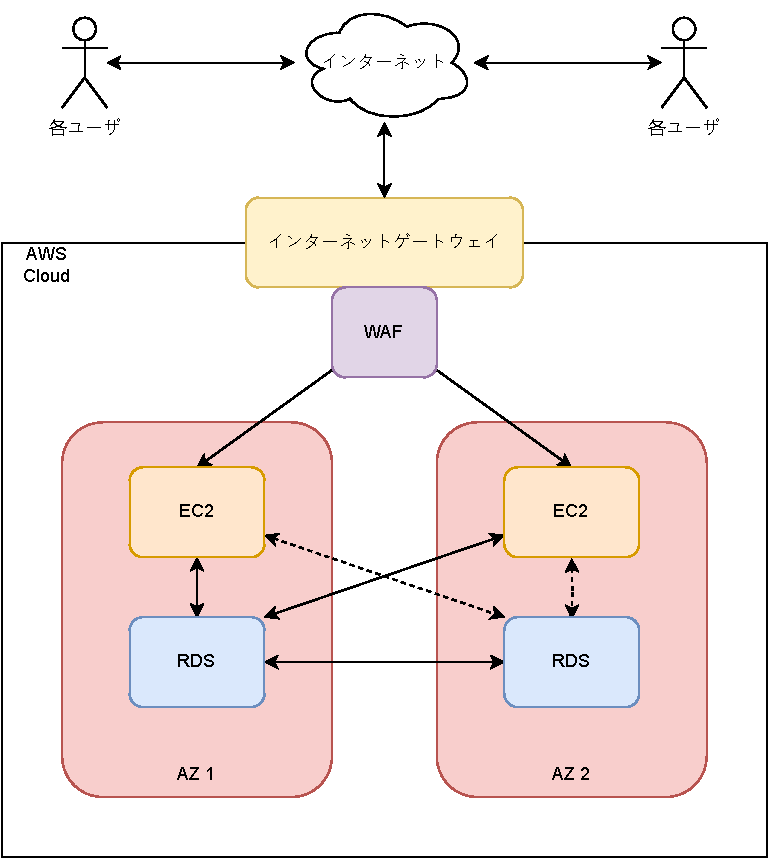
\includegraphics[width=0.8\textwidth]{./network_img.pdf}
  \caption{ネットワーク構成図}
  \label{fig:network}
\end{figure}

\section{非機能要件}
本システムが保証する非機能要件は以下の通りである.
\subsection{セキュリティ対策}
本システムでは以下のセキュリティ対策を行う.
\subsubsection{ファイアウォール}
サーバーとの通信時にAWS WAFを用いてファイアウォールを作成し不正アクセスのリスクを軽減する.
\subsubsection{権限設定}
開発・運用・保守時に適切な権限を設定することで不正アクセスされた際のリスクを軽減する.
\subsubsection{通信の暗号化}
ユーザーが本システムにアクセスする際の通信をSSL/TLSを用いて暗号化することで,通信内容の盗聴のリスクを軽減する.
\subsubsection{データベースの暗号化}
データベースに保存されるインスタンスをAWS KMS keyを用いて暗号化することで,不正アクセスされた際のリスクを軽減する.
\subsubsection{パスワードのハッシュ化}
ハッシュ化されたパスワードをデータベースに保存することで,不正アクセスによるパスワード流出のリスクを軽減する.
\subsubsection{DDoS攻撃対策}
DDoS攻撃の対策としてAWS Shieldを用いる.
\subsection{障害対策}
本システムでは以下の障害対策を行う.
\subsubsection{サーバーの冗長化}
データベースサーバーに対して可用性向上の為,プライマリ・セカンダリ構成の冗長化を行う.
\subsubsection{サーバーの負荷分散}
特定のwebサーバーに対して負荷が集中することを避けるために,ロードバランサーを用い負荷の分散を行う.
\bibliographystyle{junsrt}
\bibliography{References.bib}

\end{document}
